\section{Additional experimental results}
\label{app:additional-exp}

\paragraph{Table of results for Section~\ref{sec:rq4}}
Table~\ref{tab:rq4-main} shows the results for the \texttt{search\_commits} ablation on the set of $96$ bugs that were successfully resolved by \cresearcher{} (GPT-4o, Pass@$5$, $15$ \maxcalls{}).

\begin{table}[htp]
\centering
\caption{Importance of causal analysis of past commits on 96 bugs resolved by \cresearcher{}.}
\label{tab:rq4-main}
\begin{tabular}{ccccccc}
\cmidrule{1-7}
& \textbf{Tool} & \makecell{\textbf{Max} \\ \textbf{Calls}} & \textbf{P@k} & \textbf{CRR(\%)} & \makecell{\textbf{Avg.}\\\textbf{Recall}} & \textbf{All/Any/None(\%)}\\
\cmidrule{1-7}
& \textbf{\cresearcher{} (GPT-4o)} & $15$     & P@5  & $\mathbf{48.00}$ & $\mathbf{0.51}$ & $\mathbf{48.2} / 7.8 / 44.0$ \\
& \textsc{w/o} \texttt{search\_commits} & $15$     & P@5  & $38.00$ & $0.33$ & $32.6/2.4/65.0$ \\
\cmidrule{1-7}
\end{tabular}
\begin{flushleft}
\footnotesize{$^1$ We do this ablation only on the 96 bugs resolved by \cresearcher{}~(GPT-4o, Pass@$5$, $15$ \maxcalls{}).}
\end{flushleft}
\end{table}

\begin{figure}[htp]
    \centering
    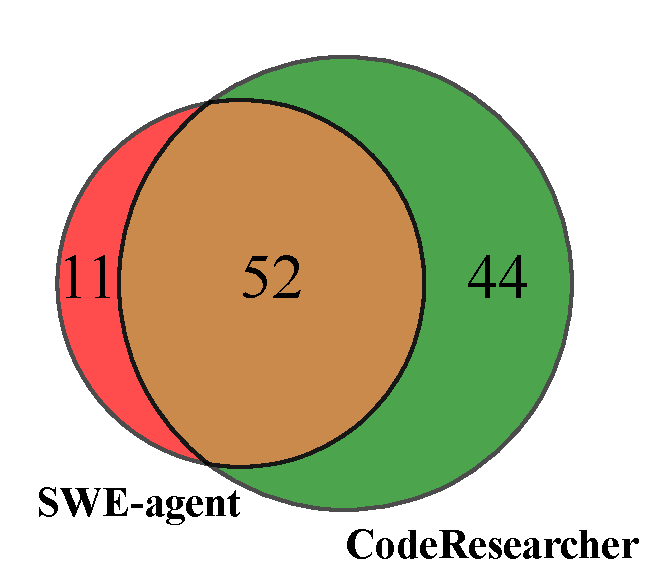
\includegraphics[scale=0.4,keepaspectratio]{images/venn_diagram.pdf}
    \caption{Overlap of crashes resolved by SWE-agent and \cresearcher{} (both at GPT-4o, P@$5$, $15$ max calls)}
    \label{fig:venn}
\end{figure}
\paragraph{Subset analysis of the crashes resolved by \cresearcher{} and SWE-agent}
Figure~\ref{fig:venn} shows a venn diagram of the crashes resolved by \cresearcher{} and SWE-agent in the same configuration (GPT-4o,P@$5$,$15$ \maxcalls{}).
It shows that \cresearcher{} is able to solve most of the crashes that SWE-agent resolves, while also resolving a significant number of additional crashes.